%!TEX root = ./FMi_2015_AISC.tex
%
% UTF8-Check: Umlaute: äöüÄÖÜß
%
\label{sec:grassintegration}
In this section, we show how the Grass GIS has been integrated in \Renew{}.
%
First, a short overview of the Grass GIS is given. 
%
This includes the Grass modules as well as the required structure of a GIS project. 
%
Next, we introduce the architecture to show all the components taking part to the integration.
%
%Somewhere here we must add the literature already published on \RenewGrass{}

\subsection{Integration Issues}
%
The first obstacle we faced when trying to integrate the Grass GIS with \Renew{} is that these tools are written in different programming languages.
(The Grass GIS is written in C and \Renew{} in Java), which makes a direct communication between them arduous.
%
Thus the Grass GIS needs to be adapted to the running environment of \Renew{}.
%
Moreover, a proper environment variables need to be pre-specified.
%
In order to achieve this integration, there are three possibilities:

\begin{itemize}
 \item
 \emph{Desktop integration}: 
 this means that the Grass GIS is locally deployed and interfaces are provided to use geoprocessing functions from \Renew{}.
\item
 \emph{Web-based integration}: 
 in this case, the objective is to publish and execute geo-processes over the web, following the Web Processing Service (WPS) interface specification\footnote{\url{http://www.opengeospatial.org/standards/wps}} from the Open Geospatial Consortium (OGC)\footnote{\url{http://www.opengeospatial.org/}}.
\item
\emph{Remote execution (Vagrant)}: 
this is another alternative to deploy the Grass GIS into the Cloud and is discussed in Section.~\ref{sec:discussion}.

\end{itemize}

%In this paper, we focus on the first solution.
%
%The integration using the WPS is here omitted but we are currently investigating this issue in another work, which concerns the perspective of moving the actual work to be executed in the cloud (see Section.~\ref{sec:discussion}).  
%
Fig.~\ref{fig:overview} is a simple overview of the integration of Grass GIS as desktop application. 
%
With \Renew{} scientific workflows are specified as Petri net models. 
%
When some of workflow tasks require Grass commands, this can be easily performed directly at the transitions.
%
In order to communicate directly with the Grass GIS, an interface or a wrapper is necessary. 

Over the last few years some effort has been dedicated to leverage the strength of Java and Grass GIS. 
%
There are some contributions dealing with this issue \cite{moldt18}. 
%
Two candidate projects are interesting for our work, which are the \textit{JGrasstools}%
\footnote{\url{http://moovida.github.io/jgrasstools/}} 
and the \textit{vtkGRASSBridge}%
\footnote{\url{https://code.google.com/p/vtk-grass-bridge/}}.
%
The \textit{vtkGRASSBridge} provides a VTK/C++ interface to most of the GIS GRASS raster, voxel and vector C library functions
%
This library can be used to build comprehensive 3D visualisation of GIS GRASS data with Java, Python and C++.
%
Although the project seems promising, it was quickly rejected, due to building issues. 
%
We realized, that future users of the tool will certainly run into similar issues, when modeling and executing workflows with \RenewGrass{} if we followed this approach.
%
For this work, we chose to take advantages from the JGrasstools project.
%
JGrasstools is a library that is extracted from the Java Geographic Resources Analysis Support System (JGrass) project.%
\footnote{JGrass is a free, multi platform, open source GIS based on the GIS framework (see \url{www.jgrass.org}).}
%

\begin{figure}[!t]
\centering
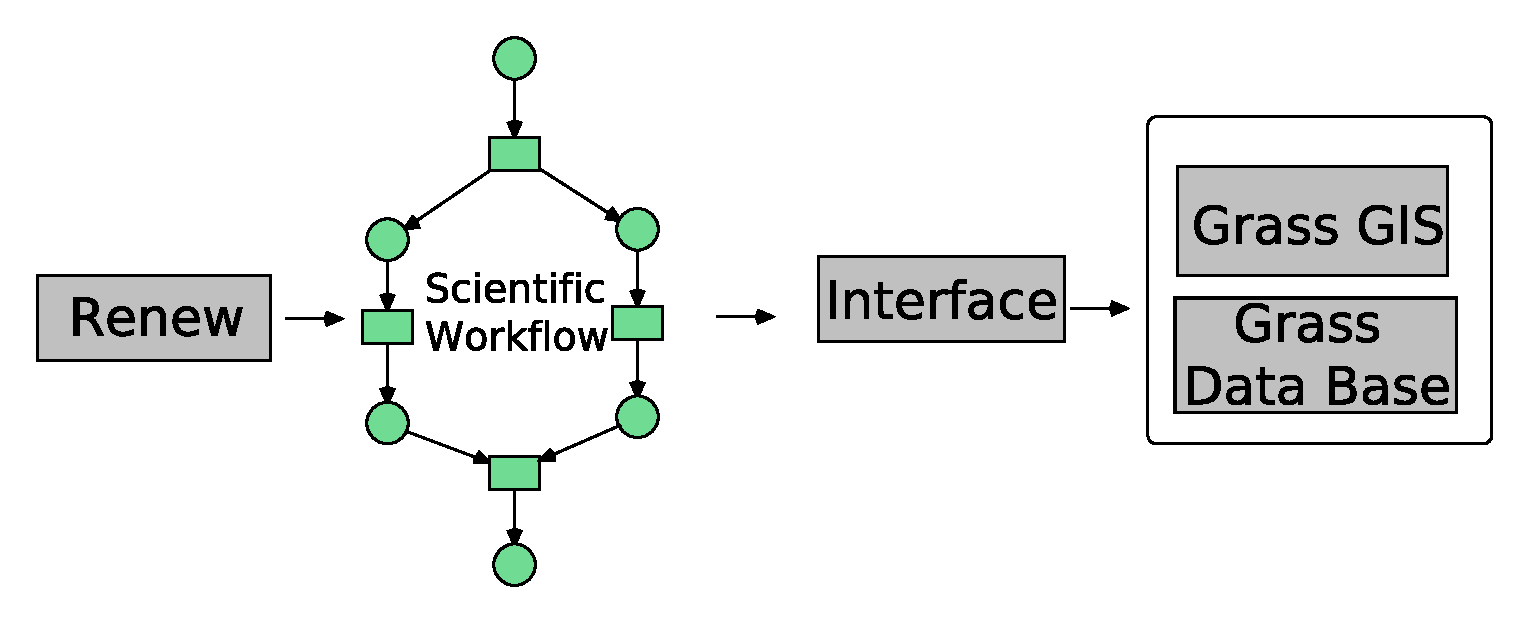
\includegraphics[width=0.78\textwidth,height=0.24\textheight]{overview}
\caption{Grass GIS Integration with \Renew{}}
\label{fig:overview}
\end{figure}


\subsection{Architecture}
\label{sec:arch}
%
As mentioned above, \Renew{}'s architecture has been decomposed into several components.
%
Each component is characterized as a plug-in.
%
This provides more flexibility and extensibility.
%
Thus new features can be easily integrated.
%
The basis for this is the \Renew{} plug-in system \cite{Duvigneau10}, which is responsible for the addition and the removal of plug-ins at runtime.


%
New features include some new plug-ins as for instance the \emph{Workflow} and the \emph{WFNet}, which provide workflow management functionality.
%
The original functionality was already presented in \cite{Jacob+02a}.
%
The \RenewGrass{} tool is also built following the plug-in architecture of \Renew{}.
%
Fig.~\ref{fig:renewgrass} shows a simplified view of the position of \RenewGrass{} in \Renew{}.
%

The \emph{Workflow} and the \emph{WFNet} plug-ins are not required when using \RenewGrass{}. 
%
They are used especially when the users want to integrate workflow management functionality such as log-in, tasks management, etc. 
%
As you can see in the figure, the \RenewGrass{} plug-in is built on top of the JGrasstools, which was adapted for \Renew{}.
%
The main requirements are the Grass GIS installation and the Grass data. 
%
The first one provides all the modules presented in Section.~\ref{subsec:grassgis}. 
%
The Grass data is a directory, that holds all the required files (raster or vector images).
%
Both Grass GIS installation and the Grass Data path should be specified to \RenewGrass{} prior any utilization.
%
The actual implementation of the tool allows local execution only, since both \Renew{} and Grass GIS are installed on-premise. 
%
The use of external resources, mainly Cloud computing resources, is not excluded, but it is out of scope of this paper.
%
\RenewGrass{} is freely available via \url{www.paose.net} and \url{http://sofianeb.github.io/}.
%


\begin{figure}[!t]
\centering
%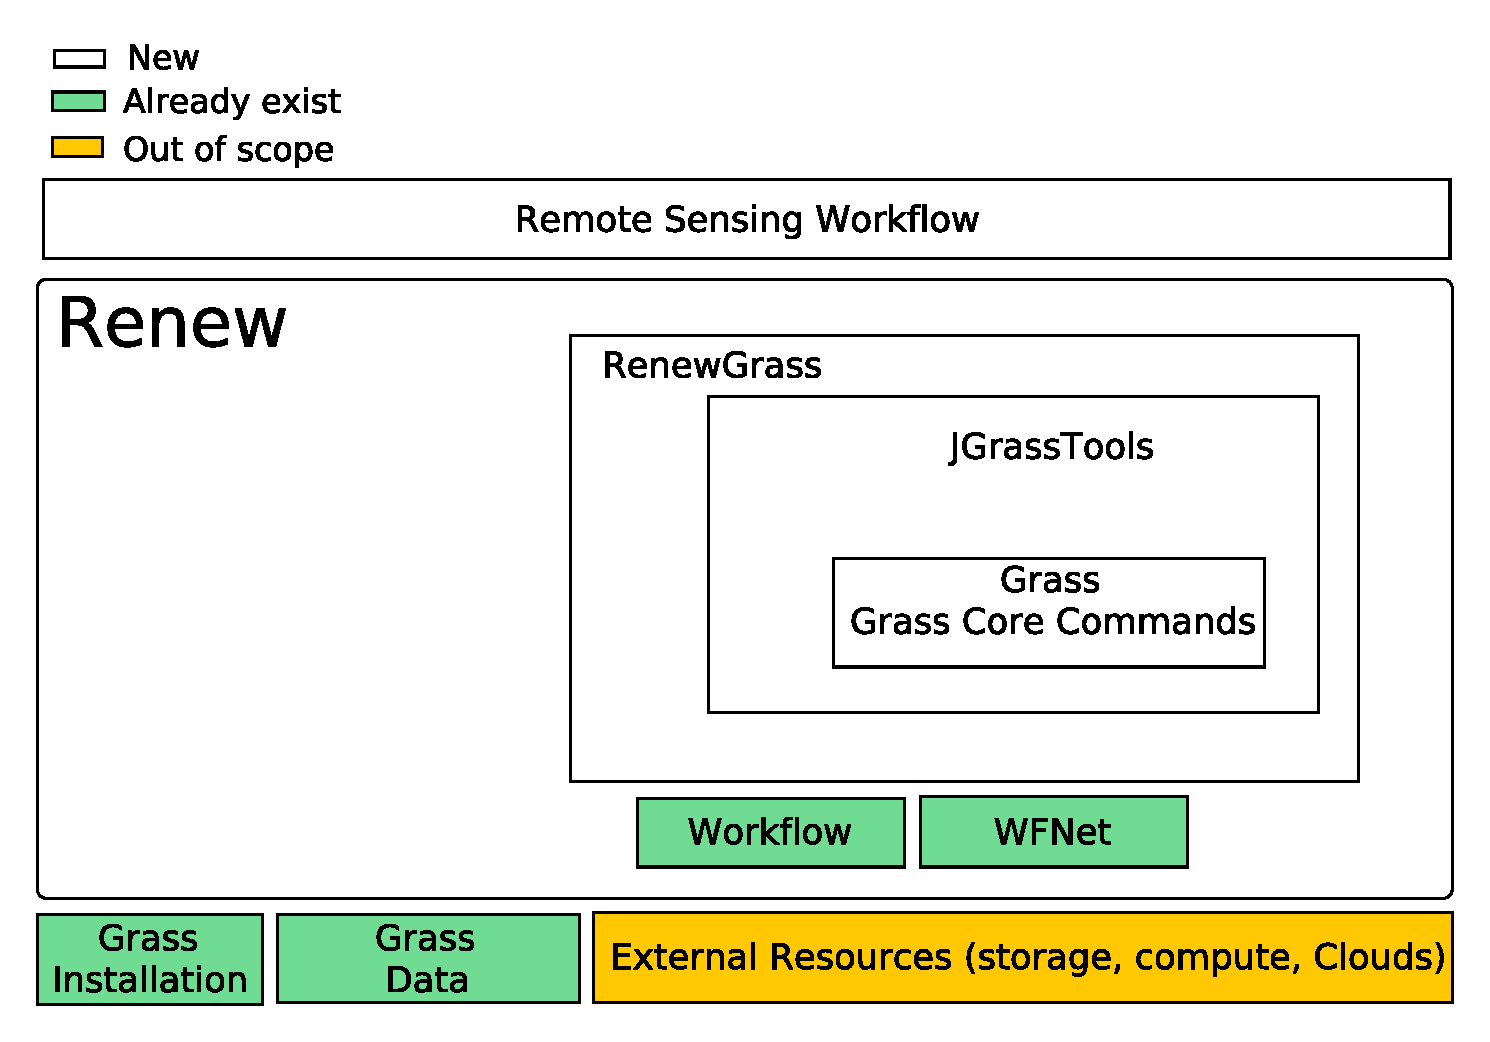
\includegraphics[width=0.78\textwidth,height=0.30\textheight]{ArchitectureGrassRenew2}
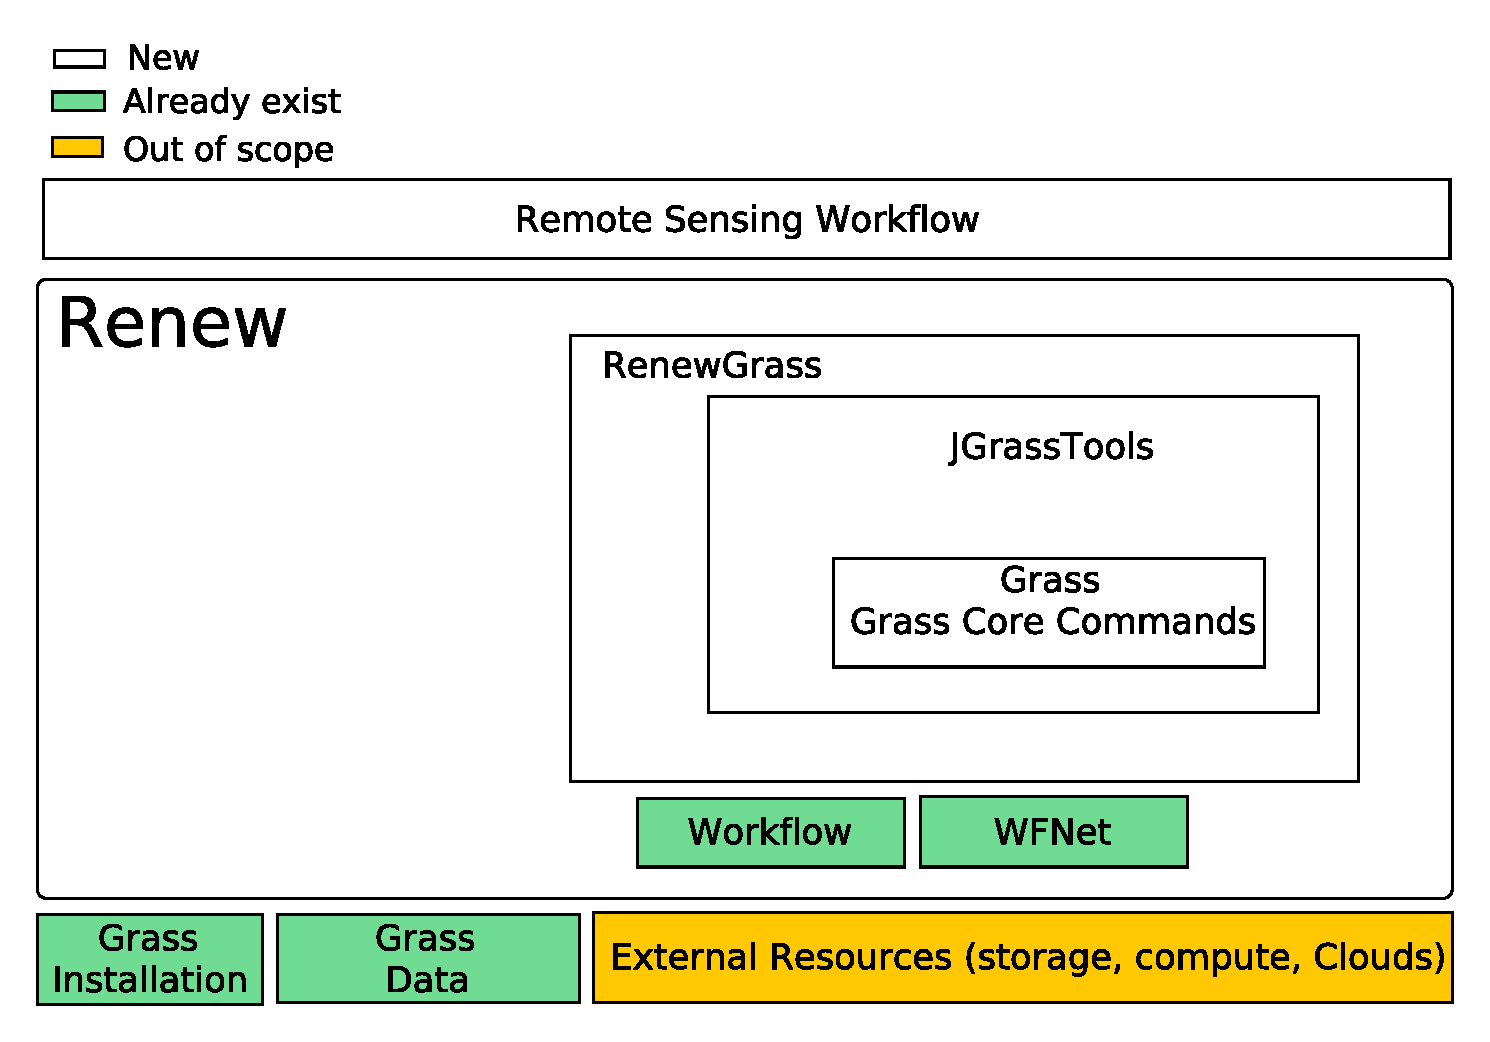
\includegraphics[width=\textwidth]{ArchitectureGrassRenew2}
\caption{Architecture of the \RenewGrass{} Tool}
\label{fig:renewgrass}
\end{figure}
%EOF



